\chapter{Quy hoạch động}

\index{dynamic programming}

\key{Quy hoạch động (Dynamic programming)}
là một kỹ thuật kết hợp tính đúng đắn
của tìm kiếm toàn bộ và hiệu quả
của các thuật toán tham lam.
Quy hoạch động có thể được áp dụng nếu bài toán
có thể được chia thành các bài toán con chồng chéo
có thể được giải quyết một cách độc lập.

Có hai ứng dụng cho quy hoạch động:

\begin{itemize}
\item
\key{Tìm một giải pháp tối ưu}:
Chúng ta muốn tìm một giải pháp
lớn nhất có thể hoặc nhỏ nhất có thể.
\item
\key{Đếm số lượng các giải pháp}:
Chúng ta muốn tính tổng số
các giải pháp có thể.
\end{itemize}

Đầu tiên, chúng ta sẽ xem quy hoạch động có thể được
sử dụng để tìm một giải pháp tối ưu như thế nào,
và sau đó chúng ta sẽ sử dụng cùng một ý tưởng để
đếm các giải pháp.

Hiểu được quy hoạch động là một cột mốc quan trọng
trong sự nghiệp của mọi lập trình viên thi đấu.
Mặc dù ý tưởng cơ bản là đơn giản,
thách thức là làm thế nào để áp dụng
quy hoạch động vào các bài toán khác nhau.
Chương này giới thiệu một tập hợp các bài toán kinh điển
là một điểm khởi đầu tốt.

\section{Bài toán đồng xu}

Đầu tiên, chúng ta tập trung vào một bài toán mà chúng ta
đã thấy trong Chương 6:
Cho một tập hợp các mệnh giá đồng xu $\texttt{coins} = \{c_1,c_2,\ldots,c_k\}$
và một tổng tiền mục tiêu $n$, nhiệm vụ của chúng ta là
tạo thành tổng $n$ bằng cách sử dụng càng ít đồng xu càng tốt.

Trong Chương 6, chúng ta đã giải quyết bài toán bằng cách sử dụng một
thuật toán tham lam luôn chọn đồng xu
lớn nhất có thể.
Thuật toán tham lam hoạt động, ví dụ,
khi các đồng xu là các đồng xu euro,
nhưng trong trường hợp tổng quát, thuật toán tham lam
không nhất thiết tạo ra một giải pháp tối ưu.

Bây giờ là lúc để giải quyết bài toán một cách hiệu quả
sử dụng quy hoạch động, sao cho thuật toán
hoạt động với bất kỳ bộ đồng xu nào.
Thuật toán quy hoạch động
dựa trên một hàm đệ quy
duyệt qua tất cả các khả năng để
tạo thành tổng, giống như một thuật toán duyệt toàn bộ.
Tuy nhiên, thuật toán quy hoạch động
hiệu quả vì
nó sử dụng \emph{ghi nhớ (memoization)} và
tính toán câu trả lời cho mỗi bài toán con chỉ một lần.

\subsubsection{Công thức đệ quy}

Ý tưởng trong quy hoạch động là
xây dựng bài toán một cách đệ quy sao cho
lời giải của bài toán có thể được
tính toán từ các lời giải của các bài toán con nhỏ hơn.
Trong bài toán đồng xu, một bài toán
đệ quy tự nhiên như sau:
số lượng đồng xu nhỏ nhất
cần thiết để tạo thành một tổng $x$ là bao nhiêu?

Gọi $\texttt{solve}(x)$
biểu thị số lượng
đồng xu tối thiểu cần thiết cho một tổng $x$.
Các giá trị của hàm phụ thuộc vào
các giá trị của các đồng xu.
Ví dụ, nếu $\texttt{coins} = \{1,3,4\}$,
các giá trị đầu tiên của hàm như sau:

\[
\begin{array}{lcl}
\texttt{solve}(0) & = & 0 \\
\texttt{solve}(1) & = & 1 \\
\texttt{solve}(2) & = & 2 \\
\texttt{solve}(3) & = & 1 \\
\texttt{solve}(4) & = & 1 \\
\texttt{solve}(5) & = & 2 \\
\texttt{solve}(6) & = & 2 \\
\texttt{solve}(7) & = & 2 \\
\texttt{solve}(8) & = & 2 \\
\texttt{solve}(9) & = & 3 \\
\texttt{solve}(10) & = & 3 \\
\end{array}
\]

Ví dụ, $\texttt{solve}(10)=3$,
bởi vì cần ít nhất 3 đồng xu
để tạo thành tổng 10.
Giải pháp tối ưu là $3+3+4=10$.

Thuộc tính thiết yếu của $\texttt{solve}$ là
các giá trị của nó có thể được
tính toán một cách đệ quy từ các giá trị nhỏ hơn của nó.
Ý tưởng là tập trung vào đồng xu \emph{đầu tiên}
mà chúng ta chọn cho tổng.
Ví dụ, trong kịch bản trên,
đồng xu đầu tiên có thể là 1, 3 hoặc 4.
Nếu chúng ta chọn đồng xu 1 đầu tiên,
nhiệm vụ còn lại là tạo thành tổng 9
sử dụng số lượng đồng xu tối thiểu,
đó là một bài toán con của bài toán ban đầu.
Tất nhiên, điều tương tự cũng áp dụng cho các đồng xu 3 và 4.
Do đó, chúng ta có thể sử dụng công thức đệ quy sau
để tính số lượng đồng xu tối thiểu:
\begin{equation*}
\begin{split}
\texttt{solve}(x) = \min( & \texttt{solve}(x-1)+1, \\
                           & \texttt{solve}(x-3)+1, \\
                           & \texttt{solve}(x-4)+1).
\end{split}
\end{equation*}
Trường hợp cơ sở của đệ quy là $\texttt{solve}(0)=0$,
bởi vì không cần đồng xu nào để tạo thành một tổng rỗng.
Ví dụ,
\[ \texttt{solve}(10) = \texttt{solve}(7)+1 = \texttt{solve}(4)+2 = \texttt{solve}(0)+3 = 3.\]

Bây giờ chúng ta sẵn sàng đưa ra một hàm đệ quy tổng quát
tính toán số lượng đồng xu
tối thiểu cần thiết để tạo thành một tổng $x$:
\begin{equation*}
    \texttt{solve}(x) = \begin{cases}
               \infty               & x < 0\\
               0               & x = 0\\
               \min_{c \in \texttt{coins}} \texttt{solve}(x-c)+1 & x > 0 \\
           \end{cases}
\end{equation*}

Đầu tiên, nếu $x<0$, giá trị là $\infty$,
bởi vì không thể tạo thành một
tổng tiền âm.
Sau đó, nếu $x=0$, giá trị là $0$,
bởi vì không cần đồng xu nào để tạo thành một tổng rỗng.
Cuối cùng, nếu $x>0$, biến $c$ duyệt qua
tất cả các khả năng để chọn đồng xu đầu tiên
của tổng.

Một khi một hàm đệ quy giải quyết được bài toán
đã được tìm thấy,
chúng ta có thể triển khai trực tiếp một giải pháp trong C++
(hằng số \texttt{INF} biểu thị vô cùng):

\begin{lstlisting}
int solve(int x) {
    if (x < 0) return INF;
    if (x == 0) return 0;
    int best = INF;
    for (auto c : coins) {
        best = min(best, solve(x-c)+1);
    }
    return best;
}
\end{lstlisting}

Tuy nhiên, hàm này không hiệu quả,
bởi vì có thể có một số lượng mũ các cách
để xây dựng tổng.
Tuy nhiên, tiếp theo chúng ta sẽ xem cách làm cho
hàm này hiệu quả bằng cách sử dụng một kỹ thuật gọi là ghi nhớ.

\subsubsection{Sử dụng ghi nhớ (memoization)}

\index{memoization}

Ý tưởng của quy hoạch động là sử dụng
\key{ghi nhớ (memoization)} để tính toán hiệu quả
các giá trị của một hàm đệ quy.
Điều này có nghĩa là các giá trị của hàm
được lưu trữ trong một mảng sau khi tính toán chúng.
Đối với mỗi tham số, giá trị của hàm
được tính toán đệ quy chỉ một lần, và sau đó,
giá trị có thể được lấy trực tiếp từ mảng.

Trong bài toán này, chúng ta sử dụng các mảng
\begin{lstlisting}
bool ready[N];
int value[N];
\end{lstlisting}

trong đó $\texttt{ready}[x]$ chỉ ra
liệu giá trị của $\texttt{solve}(x)$ đã được tính toán hay chưa,
và nếu đã được tính, $\texttt{value}[x]$
chứa giá trị này.
Hằng số $N$ đã được chọn sao cho
tất cả các giá trị cần thiết đều vừa với các mảng.

Bây giờ hàm có thể được triển khai một cách hiệu quả
như sau:

\begin{lstlisting}
int solve(int x) {
    if (x < 0) return INF;
    if (x == 0) return 0;
    if (ready[x]) return value[x];
    int best = INF;
    for (auto c : coins) {
        best = min(best, solve(x-c)+1);
    }
    value[x] = best;
    ready[x] = true;
    return best;
}
\end{lstlisting}

Hàm xử lý các trường hợp cơ sở
$x<0$ và $x=0$ như trước.
Sau đó, hàm kiểm tra từ
$\texttt{ready}[x]$ xem
$\texttt{solve}(x)$ đã được lưu trữ
trong $\texttt{value}[x]$ hay chưa,
và nếu có, hàm sẽ trả về nó trực tiếp.
Ngược lại, hàm sẽ tính giá trị
của $\texttt{solve}(x)$
một cách đệ quy và lưu nó vào $\texttt{value}[x]$.

Hàm này hoạt động hiệu quả,
bởi vì câu trả lời cho mỗi tham số $x$
được tính toán đệ quy chỉ một lần.
Sau khi một giá trị của $\texttt{solve}(x)$ đã được lưu trữ trong $\texttt{value}[x]$,
nó có thể được lấy ra một cách hiệu quả bất cứ khi nào
hàm sẽ được gọi lại với tham số $x$.
Độ phức tạp thời gian của thuật toán là $O(nk)$,
trong đó $n$ là tổng mục tiêu và $k$ là số lượng đồng xu.

Lưu ý rằng chúng ta cũng có thể xây dựng mảng \texttt{value} một cách \emph{lặp}
bằng cách sử dụng một vòng lặp chỉ đơn giản là tính toán tất cả các giá trị
của $\texttt{solve}$ cho các tham số $0 \ldots n$:
\begin{lstlisting}
value[0] = 0;
for (int x = 1; x <= n; x++) {
    value[x] = INF;
    for (auto c : coins) {
        if (x-c >= 0) {
            value[x] = min(value[x], value[x-c]+1);
        }
    }
}
\end{lstlisting}

Thực tế, hầu hết các lập trình viên thi đấu thích cách
triển khai này hơn, bởi vì nó ngắn hơn và có
các hệ số hằng thấp hơn.
Từ bây giờ, chúng ta cũng sử dụng các cách triển khai lặp
trong các ví dụ của mình.
Tuy nhiên, thường thì việc suy nghĩ về
các giải pháp quy hoạch động
dưới dạng các hàm đệ quy sẽ dễ dàng hơn.


\subsubsection{Xây dựng một giải pháp}

Đôi khi chúng ta được yêu cầu vừa tìm giá trị
của một giải pháp tối ưu vừa đưa ra
một ví dụ về cách một giải pháp như vậy có thể được xây dựng.
Trong bài toán đồng xu, ví dụ,
chúng ta có thể khai báo một mảng khác
chỉ ra cho
mỗi tổng tiền đồng xu đầu tiên 
trong một giải pháp tối ưu:
\begin{lstlisting}
int first[N];
\end{lstlisting}
Sau đó, chúng ta có thể sửa đổi thuật toán như sau:
\begin{lstlisting}
value[0] = 0;
for (int x = 1; x <= n; x++) {
    value[x] = INF;
    for (auto c : coins) {
        if (x-c >= 0 && value[x-c]+1 < value[x]) {
            value[x] = value[x-c]+1;
            first[x] = c;
        }
    }
}
\end{lstlisting}
Sau đó, đoạn mã sau có thể được sử dụng để
in ra các đồng xu xuất hiện trong một giải pháp tối ưu cho
tổng $n$:
\begin{lstlisting}
while (n > 0) {
    cout << first[n] << "\n";
    n -= first[n];
}
\end{lstlisting}

\subsubsection{Đếm số lượng các giải pháp}

Bây giờ chúng ta hãy xem xét một phiên bản khác
của bài toán đồng xu trong đó nhiệm vụ của chúng ta là
tính tổng số cách
để tạo ra một tổng $x$ bằng cách sử dụng các đồng xu.
Ví dụ, nếu $\texttt{coins}=\{1,3,4\}$ và
$x=5$, có tổng cộng 6 cách:

\begin{multicols}{2}
\begin{itemize}
\item $1+1+1+1+1$
\item $1+1+3$
\item $1+3+1$
\item $3+1+1$
\item $1+4$
\item $4+1$
\end{itemize}
\end{multicols}

Một lần nữa, chúng ta có thể giải quyết bài toán một cách đệ quy.
Gọi $\texttt{solve}(x)$ là số cách
chúng ta có thể tạo thành tổng $x$.
Ví dụ, nếu $\texttt{coins}=\{1,3,4\}$,
thì $\texttt{solve}(5)=6$ và công thức đệ quy là
\begin{equation*}
\begin{split}
\texttt{solve}(x) = & \texttt{solve}(x-1) + \\
                    & \texttt{solve}(x-3) + \\
                    & \texttt{solve}(x-4)  .
\end{split}
\end{equation*}

Sau đó, hàm đệ quy tổng quát như sau:
\begin{equation*}
    \texttt{solve}(x) = \begin{cases}
               0               & x < 0\\
               1               & x = 0\\
               \sum_{c \in \texttt{coins}} \texttt{solve}(x-c) & x > 0 \\
           \end{cases}
\end{equation*}

Nếu $x<0$, giá trị là 0, vì không có giải pháp nào.
Nếu $x=0$, giá trị là 1, vì chỉ có một cách
để tạo thành một tổng rỗng.
Ngược lại, chúng ta tính tổng của tất cả các giá trị
có dạng $\texttt{solve}(x-c)$ trong đó $c$ nằm trong \texttt{coins}.

Đoạn mã sau xây dựng một mảng
$\texttt{count}$ sao cho
$\texttt{count}[x]$ bằng
giá trị của $\texttt{solve}(x)$
cho $0 \le x \le n$:

\begin{lstlisting}
count[0] = 1;
for (int x = 1; x <= n; x++) {
    for (auto c : coins) {
        if (x-c >= 0) {
            count[x] += count[x-c];
        }
    }
}
\end{lstlisting}

Thường thì số lượng các giải pháp lớn đến mức
không cần phải tính số chính xác
mà chỉ cần đưa ra câu trả lời theo mô-đun $m$
trong đó, ví dụ, $m=10^9+7$.
Điều này có thể được thực hiện bằng cách thay đổi mã sao cho
tất cả các tính toán được thực hiện theo mô-đun $m$.
Trong đoạn mã trên, chỉ cần thêm dòng
\begin{lstlisting}
        count[x] %= m;
\end{lstlisting}
sau dòng
\begin{lstlisting}
        count[x] += count[x-c];
\end{lstlisting}

Bây giờ chúng ta đã thảo luận về tất cả các ý tưởng cơ bản
của quy hoạch động.
Vì quy hoạch động có thể được sử dụng
trong nhiều tình huống khác nhau,
bây giờ chúng ta sẽ xem xét một tập hợp các bài toán
để minh họa thêm về các
khả năng của quy hoạch động.

\section{Dãy con tăng dài nhất}

\index{longest increasing subsequence}

Bài toán đầu tiên của chúng ta là tìm
\key{dãy con tăng dài nhất (longest increasing subsequence)}
trong một mảng gồm $n$ phần tử.
Đây là một dãy có độ dài tối đa
gồm các phần tử mảng
đi từ trái sang phải,
và mỗi phần tử trong dãy lớn hơn
phần tử trước đó.
Ví dụ, trong mảng

\begin{center}
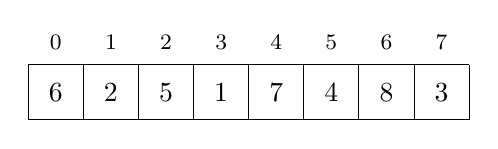
\begin{tikzpicture}[scale=0.7]
\draw (0,0) grid (8,1);
\node at (0.5,0.5) {$6$};
\node at (1.5,0.5) {$2$};
\node at (2.5,0.5) {$5$};
\node at (3.5,0.5) {$1$};
\node at (4.5,0.5) {$7$};
\node at (5.5,0.5) {$4$};
\node at (6.5,0.5) {$8$};
\node at (7.5,0.5) {$3$};

\footnotesize
\node at (0.5,1.4) {$0$};
\node at (1.5,1.4) {$1$};
\node at (2.5,1.4) {$2$};
\node at (3.5,1.4) {$3$};
\node at (4.5,1.4) {$4$};
\node at (5.5,1.4) {$5$};
\node at (6.5,1.4) {$6$};
\node at (7.5,1.4) {$7$};
\end{tikzpicture}
\end{center}
dãy con tăng dài nhất
chứa 4 phần tử:
\begin{center}
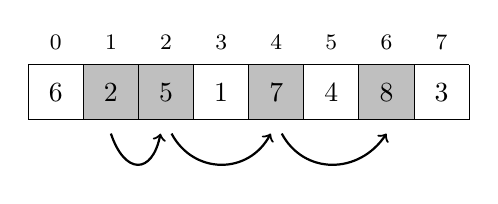
\begin{tikzpicture}[scale=0.7]
\fill[color=lightgray] (1,0) rectangle (2,1);
\fill[color=lightgray] (2,0) rectangle (3,1);
\fill[color=lightgray] (4,0) rectangle (5,1);
\fill[color=lightgray] (6,0) rectangle (7,1);
\draw (0,0) grid (8,1);
\node at (0.5,0.5) {$6$};
\node at (1.5,0.5) {$2$};
\node at (2.5,0.5) {$5$};
\node at (3.5,0.5) {$1$};
\node at (4.5,0.5) {$7$};
\node at (5.5,0.5) {$4$};
\node at (6.5,0.5) {$8$};
\node at (7.5,0.5) {$3$};

\draw[thick,->] (1.5,-0.25) .. controls (1.75,-1.00) and (2.25,-1.00) .. (2.4,-0.25);
\draw[thick,->] (2.6,-0.25) .. controls (3.0,-1.00) and (4.0,-1.00) .. (4.4,-0.25);
\draw[thick,->] (4.6,-0.25) .. controls (5.0,-1.00) and (6.0,-1.00) .. (6.5,-0.25);

\footnotesize
\node at (0.5,1.4) {$0$};
\node at (1.5,1.4) {$1$};
\node at (2.5,1.4) {$2$};
\node at (3.5,1.4) {$3$};
\node at (4.5,1.4) {$4$};
\node at (5.5,1.4) {$5$};
\node at (6.5,1.4) {$6$};
\node at (7.5,1.4) {$7$};
\end{tikzpicture}
\end{center}

Gọi $\texttt{length}(k)$ là
độ dài của
dãy con tăng dài nhất
kết thúc tại vị trí $k$.
Do đó, nếu chúng ta tính tất cả các giá trị của
$\texttt{length}(k)$ trong đó $0 \le k \le n-1$,
chúng ta sẽ tìm ra độ dài của
dãy con tăng dài nhất.
Ví dụ, các giá trị của hàm
cho mảng trên như sau:
\[
\begin{array}{lcl}
\texttt{length}(0) & = & 1 \\
\texttt{length}(1) & = & 1 \\
\texttt{length}(2) & = & 2 \\
\texttt{length}(3) & = & 1 \\
\texttt{length}(4) & = & 3 \\
\texttt{length}(5) & = & 2 \\
\texttt{length}(6) & = & 4 \\
\texttt{length}(7) & = & 2 \\
\end{array}
\]

Ví dụ, $\texttt{length}(6)=4$,
bởi vì dãy con tăng dài nhất
kết thúc tại vị trí 6 bao gồm 4 phần tử.

Để tính một giá trị của $\texttt{length}(k)$,
chúng ta nên tìm một vị trí $i<k$
mà $\texttt{array}[i]<\texttt{array}[k]$
và $\texttt{length}(i)$ lớn nhất có thể.
Khi đó chúng ta biết rằng
$\texttt{length}(k)=\texttt{length}(i)+1$,
bởi vì đây là một cách tối ưu để thêm
$\texttt{array}[k]$ vào một dãy con.
Tuy nhiên, nếu không có vị trí $i$ nào như vậy,
thì $\texttt{length}(k)=1$,
có nghĩa là dãy con chỉ chứa
$\texttt{array}[k]$.

Vì tất cả các giá trị của hàm có thể được tính
từ các giá trị nhỏ hơn của nó,
chúng ta có thể sử dụng quy hoạch động.
Trong đoạn mã sau, các giá trị
của hàm sẽ được lưu trữ trong một mảng
$\texttt{length}$.

\begin{lstlisting}
for (int k = 0; k < n; k++) {
    length[k] = 1;
    for (int i = 0; i < k; i++) {
        if (array[i] < array[k]) {
            length[k] = max(length[k],length[i]+1);
        }
    }
}
\end{lstlisting}

Đoạn mã này hoạt động trong thời gian $O(n^2)$,
bởi vì nó bao gồm hai vòng lặp lồng nhau.
Tuy nhiên, cũng có thể triển khai
việc tính toán quy hoạch động
một cách hiệu quả hơn trong thời gian $O(n \log n)$.
Bạn có thể tìm ra cách làm điều này không?

\section{Đường đi trong lưới}

Bài toán tiếp theo của chúng ta là tìm một đường đi
từ góc trên bên trái đến
góc dưới bên phải
của một lưới $n \times n$, sao cho
chúng ta chỉ di chuyển xuống và sang phải.
Mỗi ô vuông chứa một số nguyên dương,
và đường đi nên được xây dựng sao cho
tổng các giá trị dọc theo
đường đi là lớn nhất có thể.

Hình sau cho thấy một đường đi
tối ưu trong một lưới:
\begin{center}
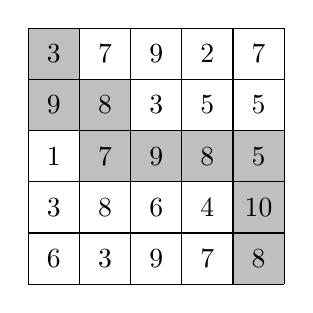
\begin{tikzpicture}[scale=.65]
  \begin{scope}
    \fill [color=lightgray] (0, 9) rectangle (1, 8);
    \fill [color=lightgray] (0, 8) rectangle (1, 7);
    \fill [color=lightgray] (1, 8) rectangle (2, 7);
    \fill [color=lightgray] (1, 7) rectangle (2, 6);
    \fill [color=lightgray] (2, 7) rectangle (3, 6);
    \fill [color=lightgray] (3, 7) rectangle (4, 6);
    \fill [color=lightgray] (4, 7) rectangle (5, 6);
    \fill [color=lightgray] (4, 6) rectangle (5, 5);
    \fill [color=lightgray] (4, 5) rectangle (5, 4);
    \draw (0, 4) grid (5, 9);
    \node at (0.5,8.5) {3};
    \node at (1.5,8.5) {7};
    \node at (2.5,8.5) {9};
    \node at (3.5,8.5) {2};
    \node at (4.5,8.5) {7};
    \node at (0.5,7.5) {9};
    \node at (1.5,7.5) {8};
    \node at (2.5,7.5) {3};
    \node at (3.5,7.5) {5};
    \node at (4.5,7.5) {5};
    \node at (0.5,6.5) {1};
    \node at (1.5,6.5) {7};
    \node at (2.5,6.5) {9};
    \node at (3.5,6.5) {8};
    \node at (4.5,6.5) {5};
    \node at (0.5,5.5) {3};
    \node at (1.5,5.5) {8};
    \node at (2.5,5.5) {6};
    \node at (3.5,5.5) {4};
    \node at (4.5,5.5) {10};
    \node at (0.5,4.5) {6};
    \node at (1.5,4.5) {3};
    \node at (2.5,4.5) {9};
    \node at (3.5,4.5) {7};
    \node at (4.5,4.5) {8};
  \end{scope}
\end{tikzpicture}
\end{center}
Tổng các giá trị trên đường đi là 67,
và đây là tổng lớn nhất có thể trên một đường đi
từ góc trên bên trái đến góc dưới bên phải.

Giả sử các hàng và các cột của
lưới được đánh số từ 1 đến $n$,
và $\texttt{value}[y][x]$ bằng giá trị
của ô vuông $(y,x)$.
Gọi $\texttt{sum}(y,x)$ là tổng
lớn nhất trên một đường đi từ góc trên bên trái
đến ô vuông $(y,x)$.
Bây giờ $\texttt{sum}(n,n)$ cho chúng ta biết
tổng lớn nhất
từ góc trên bên trái đến
góc dưới bên phải.
Ví dụ, trong lưới trên,
$\texttt{sum}(5,5)=67$.

Chúng ta có thể tính toán các tổng một cách đệ quy
như sau:
\[ \texttt{sum}(y,x) = \max(\texttt{sum}(y,x-1),\texttt{sum}(y-1,x))+\texttt{value}[y][x]\]


Công thức đệ quy dựa trên quan sát
rằng một đường đi kết thúc tại ô vuông $(y,x)$
có thể đến từ ô vuông $(y,x-1)$
hoặc ô vuông $(y-1,x)$:
\begin{center}
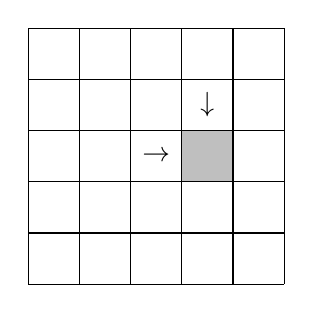
\begin{tikzpicture}[scale=.65]
  \begin{scope}
    \fill [color=lightgray] (3, 7) rectangle (4, 6);
    \draw (0, 4) grid (5, 9);
    
    \node at (2.5,6.5) {$\rightarrow$};
    \node at (3.5,7.5) {$\downarrow$};
    
  \end{scope}
\end{tikzpicture}
\end{center}

Do đó, chúng ta chọn hướng để tối đa hóa
tổng.
Chúng ta giả định rằng $\texttt{sum}(y,x)=0$
nếu $y=0$ hoặc $x=0$ (bởi vì không có đường đi nào như vậy),
vì vậy công thức đệ quy cũng hoạt động khi $y=1$ hoặc $x=1$.

Vì hàm \texttt{sum} có hai tham số,
mảng quy hoạch động cũng có hai chiều.
Ví dụ, chúng ta có thể sử dụng một mảng
\begin{lstlisting}
int sum[N][N];
\end{lstlisting}
và tính các tổng như sau:
\begin{lstlisting}
for (int y = 1; y <= n; y++) {
    for (int x = 1; x <= n; x++) {
        sum[y][x] = max(sum[y][x-1],sum[y-1][x])+value[y][x];
    }
}
\end{lstlisting}
Độ phức tạp thời gian của thuật toán là $O(n^2)$.

\section{Bài toán cái túi}

\index{knapsack}

Thuật ngữ \key{cái túi (knapsack)} đề cập đến các bài toán trong đó
một tập hợp các đồ vật được cho, và
các tập hợp con có một số thuộc tính
cần được tìm thấy.
Các bài toán cái túi thường có thể được giải quyết
bằng quy hoạch động.

Trong phần này, chúng ta tập trung vào
bài toán sau: Cho một danh sách các trọng lượng
$[w_1,w_2,\ldots,w_n]$,
xác định tất cả các
tổng có thể được xây dựng bằng cách sử dụng các trọng lượng.
Ví dụ, nếu các trọng lượng là
$[1,3,3,5]$, các tổng sau đây là có thể:

\begin{center}
\begin{tabular}{rrrrrrrrrrrrr}
 0 & 1 & 2 & 3 & 4 & 5 & 6 & 7 & 8 & 9 & 10 & 11 & 12 \\
\hline
 X & X & & X & X & X & X & X & X & X & & X & X \\
\end{tabular}
\end{center}

Trong trường hợp này, tất cả các tổng trong khoảng $0 \ldots 12$
đều có thể, ngoại trừ 2 và 10.
Ví dụ, tổng 7 là có thể vì chúng ta
có thể chọn các trọng lượng $[1,3,3]$.

Để giải quyết bài toán, chúng ta tập trung vào các bài toán con
trong đó chúng ta chỉ sử dụng $k$ trọng lượng đầu tiên
để xây dựng các tổng.
Gọi $\texttt{possible}(x,k)=\textrm{true}$ nếu
chúng ta có thể xây dựng một tổng $x$
sử dụng $k$ trọng lượng đầu tiên,
và ngược lại $\texttt{possible}(x,k)=\textrm{false}$.
Các giá trị của hàm có thể được tính
một cách đệ quy như sau:
\[ \texttt{possible}(x,k) = \texttt{possible}(x-w_k,k-1) \lor \texttt{possible}(x,k-1) \]
Công thức dựa trên thực tế là chúng ta có thể
sử dụng hoặc không sử dụng trọng lượng $w_k$ trong tổng.
Nếu chúng ta sử dụng $w_k$, nhiệm vụ còn lại là
tạo thành tổng $x-w_k$ bằng cách sử dụng $k-1$ trọng lượng đầu tiên,
và nếu chúng ta không sử dụng $w_k$,
nhiệm vụ còn lại là tạo thành tổng $x$
bằng cách sử dụng $k-1$ trọng lượng đầu tiên.
Là các trường hợp cơ sở,
\begin{equation*}
    \texttt{possible}(x,0) = \begin{cases}
               \textrm{true}    & x = 0\\
               \textrm{false}   & x \neq 0 \\
           \end{cases}
\end{equation*}
bởi vì nếu không có trọng lượng nào được sử dụng,
chúng ta chỉ có thể tạo thành tổng 0.

Bảng sau cho thấy tất cả các giá trị của hàm
cho các trọng lượng $[1,3,3,5]$ (ký hiệu "X"
chỉ ra các giá trị đúng):

\begin{center}
\begin{tabular}{r|rrrrrrrrrrrrr}
$k \backslash x$ & 0 & 1 & 2 & 3 & 4 & 5 & 6 & 7 & 8 & 9 & 10 & 11 & 12 \\
\hline
 0 & X & \\
 1 & X & X \\
 2 & X & X & & X & X \\
 3 & X & X & & X & X & & X & X \\
 4 & X & X & & X & X & X & X & X & X & X & & X & X \\
\end{tabular}
\end{center}

Sau khi tính các giá trị đó, $\texttt{possible}(x,n)$
cho chúng ta biết liệu chúng ta có thể xây dựng một
tổng $x$ bằng cách sử dụng \emph{tất cả} các trọng lượng hay không.

Gọi $W$ là tổng trọng lượng của các trọng lượng.
Giải pháp quy hoạch động thời gian $O(nW)$ sau
tương ứng với hàm đệ quy:
\begin{lstlisting}
possible[0][0] = true;
for (int k = 1; k <= n; k++) {
    for (int x = 0; x <= W; x++) {
        if (x-w[k] >= 0) possible[x][k] |= possible[x-w[k]][k-1];
        possible[x][k] |= possible[x][k-1];
    }
}
\end{lstlisting}

Tuy nhiên, đây là một cách triển khai tốt hơn chỉ sử dụng
một mảng một chiều $\texttt{possible}[x]$
chỉ ra liệu chúng ta có thể xây dựng một tập hợp con với tổng $x$ hay không.
Bí quyết là cập nhật mảng từ phải sang trái cho
mỗi trọng lượng mới:
\begin{lstlisting}
possible[0] = true;
for (int k = 1; k <= n; k++) {
    for (int x = W; x >= 0; x--) {
        if (possible[x]) possible[x+w[k]] = true;
    }
}
\end{lstlisting}

Lưu ý rằng ý tưởng chung được trình bày ở đây có thể được sử dụng
trong nhiều bài toán cái túi.
Ví dụ, nếu chúng ta được cho các đồ vật có trọng lượng và giá trị,
chúng ta có thể xác định cho mỗi tổng trọng lượng tổng giá trị
tối đa của một tập hợp con.

\section{Khoảng cách chỉnh sửa}

\index{edit distance}
\index{Levenshtein distance}

\key{Khoảng cách chỉnh sửa (edit distance)} hoặc \key{khoảng cách Levenshtein (Levenshtein distance)}\footnote{Khoảng cách
được đặt theo tên của V. I. Levenshtein, người đã nghiên cứu nó liên quan đến các mã nhị phân \cite{lev66}.}
là số lượng tối thiểu các thao tác chỉnh sửa
cần thiết để biến một chuỗi
thành một chuỗi khác.
Các thao tác chỉnh sửa được phép như sau:
\begin{itemize}
\item chèn một ký tự (ví dụ \texttt{ABC} $\rightarrow$ \texttt{ABCA})
\item xóa một ký tự (ví dụ \texttt{ABC} $\rightarrow$ \texttt{AC})
\item sửa đổi một ký tự (ví dụ \texttt{ABC} $\rightarrow$ \texttt{ADC})
\end{itemize}

Ví dụ, khoảng cách chỉnh sửa giữa
\texttt{LOVE} và \texttt{MOVIE} là 2,
bởi vì chúng ta có thể thực hiện thao tác
 \texttt{LOVE} $\rightarrow$ \texttt{MOVE}
(sửa đổi) trước và sau đó là thao tác
\texttt{MOVE} $\rightarrow$ \texttt{MOVIE}
(chèn).
Đây là số lượng thao tác nhỏ nhất có thể,
bởi vì rõ ràng là chỉ một thao tác là không đủ.

Giả sử chúng ta được cho một chuỗi \texttt{x}
có độ dài $n$ và một chuỗi \texttt{y} có độ dài $m$,
và chúng ta muốn tính khoảng cách chỉnh sửa giữa
\texttt{x} và \texttt{y}.
Để giải quyết bài toán, chúng ta định nghĩa một hàm
$\texttt{distance}(a,b)$ cho
khoảng cách chỉnh sửa giữa các tiền tố
$\texttt{x}[0 \ldots a]$ và $\texttt{y}[0 \ldots b]$.
Do đó, sử dụng hàm này, khoảng cách chỉnh sửa
giữa \texttt{x} và \texttt{y} bằng $\texttt{distance}(n-1,m-1)$.

Chúng ta có thể tính các giá trị của \texttt{distance}
như sau:
\begin{equation*}
\begin{split}
\texttt{distance}(a,b) = \min(& \texttt{distance}(a,b-1)+1, \\
                           & \texttt{distance}(a-1,b)+1, \\
                           & \texttt{distance}(a-1,b-1)+\texttt{cost}(a,b)).
\end{split}
\end{equation*}
Ở đây $\texttt{cost}(a,b)=0$ nếu $\texttt{x}[a]=\texttt{y}[b]$,
và ngược lại $\texttt{cost}(a,b)=1$.
Công thức xem xét các cách sau để
chỉnh sửa chuỗi \texttt{x}:
\begin{itemize}
\item $\texttt{distance}(a,b-1)$: chèn một ký tự vào cuối \texttt{x}
\item $\texttt{distance}(a-1,b)$: xóa ký tự cuối cùng khỏi \texttt{x}
\item $\texttt{distance}(a-1,b-1)$: khớp hoặc sửa đổi ký tự cuối cùng của \texttt{x}
\end{itemize}
Trong hai trường hợp đầu tiên, cần một thao tác chỉnh sửa
(chèn hoặc xóa).
Trong trường hợp cuối cùng, nếu $\texttt{x}[a]=\texttt{y}[b]$,
chúng ta có thể khớp các ký tự cuối cùng mà không cần chỉnh sửa,
và ngược lại cần một thao tác chỉnh sửa (sửa đổi).

Bảng sau cho thấy các giá trị của \texttt{distance}
trong trường hợp ví dụ:
\begin{center}
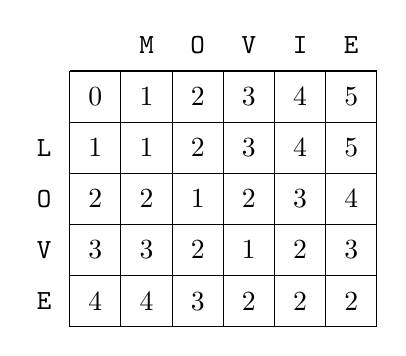
\begin{tikzpicture}[scale=.65]
  \begin{scope}
    \draw (1, -1) grid (7, -6);
    
    \node at (0.5,-2.5) {\texttt{L}};
    \node at (0.5,-3.5) {\texttt{O}};
    \node at (0.5,-4.5) {\texttt{V}};
    \node at (0.5,-5.5) {\texttt{E}};

    \node at (2.5,-0.5) {\texttt{M}};
    \node at (3.5,-0.5) {\texttt{O}};
    \node at (4.5,-0.5) {\texttt{V}};
    \node at (5.5,-0.5) {\texttt{I}};
    \node at (6.5,-0.5) {\texttt{E}};

    \node at (1.5,-1.5) {$0$};
    \node at (1.5,-2.5) {$1$};
    \node at (1.5,-3.5) {$2$};
    \node at (1.5,-4.5) {$3$};
    \node at (1.5,-5.5) {$4$};
    \node at (2.5,-1.5) {$1$};
    \node at (2.5,-2.5) {$1$};
    \node at (2.5,-3.5) {$2$};
    \node at (2.5,-4.5) {$3$};
    \node at (2.5,-5.5) {$4$};
    \node at (3.5,-1.5) {$2$};
    \node at (3.5,-2.5) {$2$};
    \node at (3.5,-3.5) {$1$};
    \node at (3.5,-4.5) {$2$};
    \node at (3.5,-5.5) {$3$};
    \node at (4.5,-1.5) {$3$};
    \node at (4.5,-2.5) {$3$};
    \node at (4.5,-3.5) {$2$};
    \node at (4.5,-4.5) {$1$};
    \node at (4.5,-5.5) {$2$};
    \node at (5.5,-1.5) {$4$};
    \node at (5.5,-2.5) {$4$};
    \node at (5.5,-3.5) {$3$};
    \node at (5.5,-4.5) {$2$};
    \node at (5.5,-5.5) {$2$};
    \node at (6.5,-1.5) {$5$};
    \node at (6.5,-2.5) {$5$};
    \node at (6.5,-3.5) {$4$};
    \node at (6.5,-4.5) {$3$};
    \node at (6.5,-5.5) {$2$};
  \end{scope}
\end{tikzpicture}
\end{center}

Góc dưới bên phải của bảng
cho chúng ta biết rằng khoảng cách chỉnh sửa giữa
\texttt{LOVE} và \texttt{MOVIE} là 2.
Bảng cũng cho thấy cách xây dựng
chuỗi thao tác chỉnh sửa ngắn nhất.
Trong trường hợp này, đường đi như sau:

\begin{center}
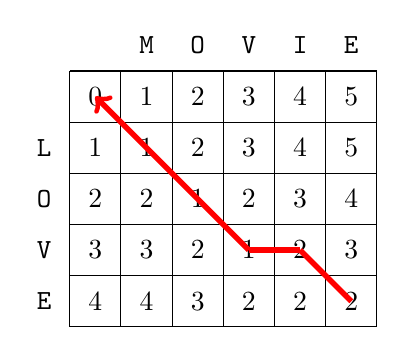
\begin{tikzpicture}[scale=.65]
  \begin{scope}
    \draw (1, -1) grid (7, -6);
    
    \node at (0.5,-2.5) {\texttt{L}};
    \node at (0.5,-3.5) {\texttt{O}};
    \node at (0.5,-4.5) {\texttt{V}};
    \node at (0.5,-5.5) {\texttt{E}};

    \node at (2.5,-0.5) {\texttt{M}};
    \node at (3.5,-0.5) {\texttt{O}};
    \node at (4.5,-0.5) {\texttt{V}};
    \node at (5.5,-0.5) {\texttt{I}};
    \node at (6.5,-0.5) {\texttt{E}};

    \node at (1.5,-1.5) {$0$};
    \node at (1.5,-2.5) {$1$};
    \node at (1.5,-3.5) {$2$};
    \node at (1.5,-4.5) {$3$};
    \node at (1.5,-5.5) {$4$};
    \node at (2.5,-1.5) {$1$};
    \node at (2.5,-2.5) {$1$};
    \node at (2.5,-3.5) {$2$};
    \node at (2.5,-4.5) {$3$};
    \node at (2.5,-5.5) {$4$};
    \node at (3.5,-1.5) {$2$};
    \node at (3.5,-2.5) {$2$};
    \node at (3.5,-3.5) {$1$};
    \node at (3.5,-4.5) {$2$};
    \node at (3.5,-5.5) {$3$};
    \node at (4.5,-1.5) {$3$};
    \node at (4.5,-2.5) {$3$};
    \node at (4.5,-3.5) {$2$};
    \node at (4.5,-4.5) {$1$};
    \node at (4.5,-5.5) {$2$};
    \node at (5.5,-1.5) {$4$};
    \node at (5.5,-2.5) {$4$};
    \node at (5.5,-3.5) {$3$};
    \node at (5.5,-4.5) {$2$};
    \node at (5.5,-5.5) {$2$};
    \node at (6.5,-1.5) {$5$};
    \node at (6.5,-2.5) {$5$};
    \node at (6.5,-3.5) {$4$};
    \node at (6.5,-4.5) {$3$};
    \node at (6.5,-5.5) {$2$};

    \path[draw=red,thick,-,line width=2pt] (6.5,-5.5) -- (5.5,-4.5);
    \path[draw=red,thick,-,line width=2pt] (5.5,-4.5) -- (4.5,-4.5);
    \path[draw=red,thick,->,line width=2pt] (4.5,-4.5) -- (1.5,-1.5);
  \end{scope}
\end{tikzpicture}
\end{center}

Các ký tự cuối cùng của \texttt{LOVE} và \texttt{MOVIE}
bằng nhau, vì vậy khoảng cách chỉnh sửa giữa chúng
bằng khoảng cách chỉnh sửa giữa \texttt{LOV} và \texttt{MOVI}.
Chúng ta có thể sử dụng một thao tác chỉnh sửa để xóa
ký tự \texttt{I} khỏi \texttt{MOVI}.
Do đó, khoảng cách chỉnh sửa lớn hơn một so với
khoảng cách chỉnh sửa giữa \texttt{LOV} và \texttt{MOV}, v.v.

\section{Đếm số cách lát gạch}

Đôi khi các trạng thái của một giải pháp quy hoạch động
phức tạp hơn các tổ hợp cố định của các số.
Ví dụ,
hãy xem xét bài toán tính
số cách khác nhau để
lấp đầy một lưới $n \times m$ bằng cách sử dụng
các viên gạch kích thước $1 \times 2$ và $2 \times 1$.
Ví dụ, một giải pháp hợp lệ
cho lưới $4 \times 7$ là
\begin{center}
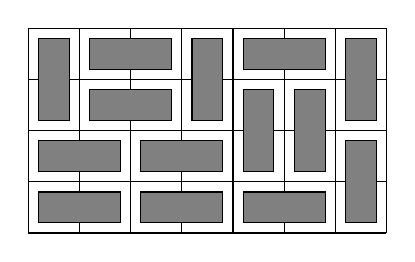
\begin{tikzpicture}[scale=.65]
    \draw (0,0) grid (7,4);
    \draw[fill=gray] (0+0.2,0+0.2) rectangle (2-0.2,1-0.2);
    \draw[fill=gray] (2+0.2,0+0.2) rectangle (4-0.2,1-0.2);
    \draw[fill=gray] (4+0.2,0+0.2) rectangle (6-0.2,1-0.2);
    \draw[fill=gray] (0+0.2,1+0.2) rectangle (2-0.2,2-0.2);
    \draw[fill=gray] (2+0.2,1+0.2) rectangle (4-0.2,2-0.2);
    \draw[fill=gray] (1+0.2,2+0.2) rectangle (3-0.2,3-0.2);
    \draw[fill=gray] (1+0.2,3+0.2) rectangle (3-0.2,4-0.2);
    \draw[fill=gray] (4+0.2,3+0.2) rectangle (6-0.2,4-0.2);

    \draw[fill=gray] (0+0.2,2+0.2) rectangle (1-0.2,4-0.2);
    \draw[fill=gray] (3+0.2,2+0.2) rectangle (4-0.2,4-0.2);
    \draw[fill=gray] (6+0.2,2+0.2) rectangle (7-0.2,4-0.2);
    \draw[fill=gray] (4+0.2,1+0.2) rectangle (5-0.2,3-0.2);
    \draw[fill=gray] (5+0.2,1+0.2) rectangle (6-0.2,3-0.2);
    \draw[fill=gray] (6+0.2,0+0.2) rectangle (7-0.2,2-0.2);

\end{tikzpicture}
\end{center}
và tổng số giải pháp là 781.

Bài toán có thể được giải quyết bằng quy hoạch động
bằng cách duyệt qua lưới từng hàng một.
Mỗi hàng trong một giải pháp có thể được biểu diễn dưới dạng một
chuỗi chứa $m$ ký tự từ tập hợp
$\{\sqcap, \sqcup, \sqsubset, \sqsupset \}$.
Ví dụ, giải pháp trên bao gồm bốn hàng
tương ứng với các chuỗi sau:
\begin{itemize}
\item
$\sqcap \sqsubset \sqsupset \sqcap \sqsubset \sqsupset \sqcap$
\item
$\sqcup \sqsubset \sqsupset \sqcup \sqcap \sqcap \sqcup$
\item
$\sqsubset \sqsupset \sqsubset \sqsupset \sqcup \sqcup \sqcap$ 
\item
$\sqsubset \sqsupset \sqsubset \sqsupset \sqsubset \sqsupset \sqcup$
\end{itemize}

Gọi $\texttt{count}(k,x)$ là số cách để
xây dựng một giải pháp cho các hàng $1 \ldots k$
của lưới sao cho chuỗi $x$ tương ứng với hàng $k$.
Có thể sử dụng quy hoạch động ở đây,
bởi vì trạng thái của một hàng chỉ bị ràng buộc
bởi trạng thái của hàng trước đó.

Một giải pháp hợp lệ nếu hàng $1$ không chứa
ký tự $\sqcup$,
hàng $n$ không chứa ký tự $\sqcap$,
và tất cả các hàng liên tiếp đều \emph{tương thích}.
Ví dụ, các hàng
$\sqcup \sqsubset \sqsupset \sqcup \sqcap \sqcap \sqcup$ và
$\sqsubset \sqsupset \sqsubset \sqsupset \sqcup \sqcup \sqcap$ 
là tương thích, trong khi các hàng
$\sqcap \sqsubset \sqsupset \sqcap \sqsubset \sqsupset \sqcap$ và
$\sqsubset \sqsupset \sqsubset \sqsupset \sqsubset \sqsupset \sqcup$
không tương thích.

Vì một hàng bao gồm $m$ ký tự và có
bốn lựa chọn cho mỗi ký tự, số lượng
hàng phân biệt nhiều nhất là $4^m$.
Do đó, độ phức tạp thời gian của giải pháp là
$O(n 4^{2m})$ bởi vì chúng ta có thể duyệt qua
$O(4^m)$ trạng thái có thể có cho mỗi hàng,
và đối với mỗi trạng thái, có $O(4^m)$
trạng thái có thể có cho hàng trước đó.
Trong thực tế, một ý tưởng tốt là xoay lưới
sao cho cạnh ngắn hơn có độ dài $m$,
bởi vì hệ số $4^{2m}$ chiếm ưu thế trong độ phức tạp thời gian.

Có thể làm cho giải pháp hiệu quả hơn
bằng cách sử dụng một biểu diễn gọn hơn cho các hàng.
Hóa ra chỉ cần biết
các cột nào của hàng trước đó chứa
ô vuông phía trên của một viên gạch dọc.
Do đó, chúng ta có thể biểu diễn một hàng chỉ bằng cách sử dụng các ký tự
$\sqcap$ và $\Box$, trong đó $\Box$ là một sự kết hợp
của các ký tự
$\sqcup$, $\sqsubset$ và $\sqsupset$.
Sử dụng biểu diễn này, chỉ có
$2^m$ hàng phân biệt và độ phức tạp thời gian là
$O(n 2^{2m})$.

Lưu ý cuối cùng, cũng có một công thức trực tiếp đáng ngạc nhiên
để tính số lượng các cách lát gạch\footnote{Đáng ngạc nhiên,
công thức này được khám phá vào năm 1961 bởi hai nhóm nghiên cứu \cite{kas61,tem61}
làm việc độc lập.}:
\[ \prod_{a=1}^{\lceil n/2 \rceil} \prod_{b=1}^{\lceil m/2 \rceil} 4 \cdot (\cos^2 \frac{\pi a}{n + 1} + \cos^2 \frac{\pi b}{m+1})\]
Công thức này rất hiệu quả, bởi vì nó tính
số lượng các cách lát gạch trong thời gian $O(nm)$,
nhưng vì câu trả lời là một tích của các số thực,
một vấn đề khi sử dụng công thức là
làm thế nào để lưu trữ các kết quả trung gian một cách chính xác.